%
% Sample SBC book chapter
%
% This is a public-domain file.
%
% Charset: ISO8859-1 (latin-1) áéíóúç
%
\documentclass{SBCbookchapter}
\usepackage[utf8]{inputenc}
\usepackage[T1]{fontenc}
\usepackage[english]{babel}
\usepackage{graphicx}
\usepackage{hyperref}
\usepackage{amsmath}
\usepackage{amsfonts}
%\usepackage{indentfirst}


\hypersetup{
colorlinks=true,
linkcolor=black,
urlcolor=blue,
citecolor = black
}

\urlstyle{same}

\usepackage{setspace}




\author{Sydney Edwards}
\title{Lost in Translation: How the Math Behind Language Models is Revolutionizing Biology}


\usepackage{lastpage}
\usepackage{fancyhdr}
\pagestyle{fancy}
\fancyhf{} % clear existing header/footer entries
% Place Page X of Y on the right-hand
% side of the footer
\fancyfoot[R]{Page \thepage \hspace{1pt} of \pageref{LastPage}}

\renewcommand{\maketitle}{%
	\noindent%
	% {\titlesize\textbf{\@title}\\[4ex]}
	% {\authorsize\@author\\[4ex]}
}


\begin{document}

\newcommand*{\getTitleGer}{\noindent Lost in Translation: How the Math Behind \\ Language Models is Revolutionizing Biology}

\newcommand*{\getauthor}{\noindent Sydney Edwards}

\makeatletter
% \centering

\vspace{4cm}
{\fontsize{\@xxpt}{23}\selectfont \bfseries \getTitleGer \par}

\vspace{0.5cm}
{\fontsize{16}\selectfont \bfseries \getauthor\par}

\maketitle

\bigskip
\bigskip
\bigskip 

\onehalfspacing

\section{Introduction}

\par The cells inside your body are decision makers \textemdash everything they do must be perfectly calibrated, perfectly timed, and in perfect coordination with the cells around them. To carry out 
their tasks, cells use proteins, building blocks of the cell that can also serve as signals to coordinate with other cells. This kind of coordination, as could be expected for any smooth operation, 
requires language. Language that says: make this protein at this time to this amount, oh and don’t forget to add a little extra leucine\footnote{Leucine is a common amino acid that is used to build 
proteins} this time. We call the language which determines the interactions inside a cell DNA. Much like the languages you’re used to, this DNA is prone to typos, grammatical errors, and complete 
nonsense\footnote{For further reading on complete nonsense found within the English language, see \url{https://twitter.com/}}, but more on why this analogy makes sense later \cite{ferruz_towards_2022}. 

For some added context, it’s helpful to know how a biology lab operates. A typical biology lab usually explores answers to the natural world by a familiar process: proof by contradiction. We wish to 
prove a gene is important for a particular process. So, assume no gene \textemdash delete it from the DNA. Then, show that the process you’re interested in has suddenly gone haywire. But we assumed that 
this gene was not important for the process, a contradiction. Thus, our gene is central to the process we wanted to initially investigate. In this whole schema, DNA is merely a means to an end 
\textemdash play with it just enough so that you can prove the assumption you wish. But DNA is so much more than a means to an end \textemdash it is the language underpinning biology that makes life 
happen. Recent work in the field of theoretical biology has begun to use concepts from linguistics, computer science, and mathematics to interrogate DNA’s properties as a language. Treating DNA as a 
language provides insight into how cells operate and coordinate with one another and how to produce novel proteins that haven’t yet popped up in the evolutionary timescale. In this paper, we’ll examine 
the history of the linguistics of DNA and the mathematics behind recent advances in the field. Ultimately we wish to demonstrate why examining DNA as a language is useful, how this is done, and what the 
next steps are for this field. 


\section{Everything You Forgot From Bio 1}

Information inside a cell always follows the same flow: DNA becomes amino acids which become proteins. We call this the central dogma of biology. The important piece is that the final proteins are 3D. 
The amino acid sequence is known as the primary structure. It is just a string of characters that biologists call a peptide. Different amino acids in this peptide interact differently with each other. 
This results in local patterns and folds within the protein. We call this the secondary structure. A secondary structure is just a description of a local topology that arises because certain amino acids 
play nice and like to fold with other amino acids. Changes in this secondary structure result in global changes to the whole protein which we conveniently call the tertiary structure. Once you know the 
secondary structure, the local topology fixes the tertiary structure and it becomes easier to predict the final protein \cite{fleming_secondary_2006}. For a visual of this process, see 
Figure~\ref{figone}. 

\begin{figure}[h!]
	\centerline{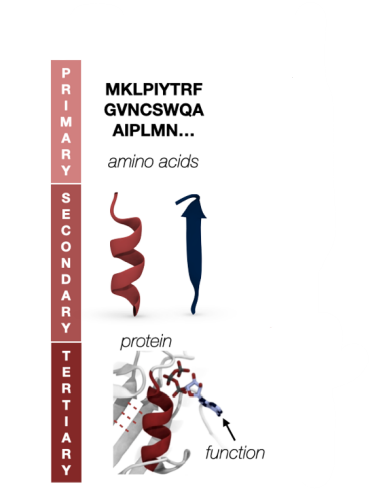
\includegraphics{rob_long_1.png}}
	\caption{The flow of information from primary to secondary to tertiary structure of peptide sequences. Figure taken from \cite{ferruz_towards_2022}. }
	\label{figone}
\end{figure}

To sum up: peptide sequences are strings of amino acids (primary structure) that fold (secondary structure) with themselves to create proteins (tertiary structure). So, why does this concept even 
matter? The amino acid sequence provides clues to the final protein structure and, due to advances in sequencing, is relatively inexpensive to find. Thus, there are rapidly expanding databases 
containing these sequences but not the final protein structure. Enter computational biologists who like working with big data. Protein structure prediction provides a unique challenge in the amount of 
unlabeled data in the training set \textemdash we simply do not know what many proteins do or what many proteins look like \cite{bepler_learning_2021}. Thus, it becomes difficult to always know whether 
our models are working, especially for the proteins that we haven’t characterized. For a pithy explanation of why the problem of protein structure prediction is challenging, see Figure~\ref{figtwo}. 

\begin{figure}[h!]
	\centerline{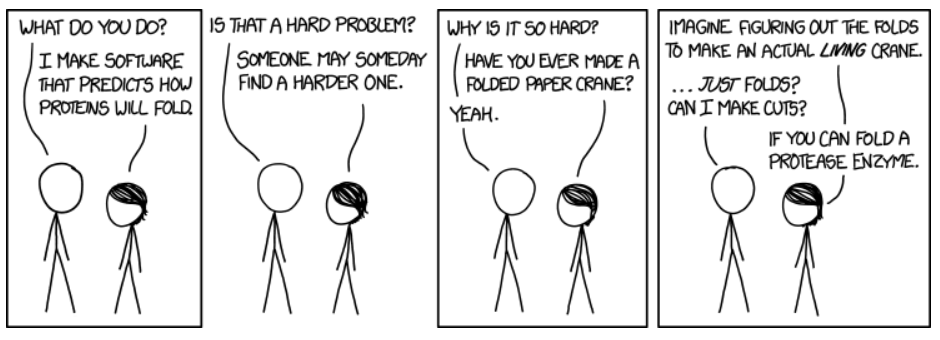
\includegraphics[scale=0.7]{rob_long_2.png}}
	\caption{Topologically determining protein structure is difficult. By formulating protein folding first as a language problem and then attempting to solve the topology of a protein, we eliminate 
some of the headache involved in fully characterizing all topological properties of proteins. This concept is known as transfer learning. Comic taken from xkcd \cite{munroe_proteins_2014}.}
	\label{figtwo}
\end{figure}

One overarching principle within biology is that form follows function. If you know the structure or form of a molecule, cell, or organ, you can readily infer what that thing can or cannot do. For 
instance, certain proteins are hydrophobic or water-hating while others are hydrophilic or water-loving, which can inform where in the cell they are found. Thus, theoretically by understanding the 
structure of a protein, you can better understand how that protein works. In a practical sense, this means that you might be able to understand how a protein works to cause a disease or how a medication 
might target a protein in the body. Additionally, understanding protein structure helps to solve one of the major problems of modern medicine \textemdash side effects. Even after medications are 
approved, new, and possibly dangerous, side effects are still reported. Almost one-third of drugs approved between 2001 and 2010 caused unexpected side effects \cite{noauthor_third_2017}. With knowledge 
of a protein's structure, we can determine whether a medication will interact with proteins of interest, including proteins in the body that we don’t want to target which could lead to nasty side 
effects \cite{mizutani_relating_2012}. Protein structure prediction ultimately helps us to better understand what goes on in the body to inform future research and possible new therapies. 

\section{Proteins, Language, and Math, Oh My}

The alphabet of proteins consists of the characters within a peptide chain \textemdash all $20$ amino acids. For an $n$-length peptide, there are thus $20^n$ possible peptides that can be made. 
Similarly, in the English language, for a $k$-length word, there are $26^k$ possible words that can be made. As described by Furruz et al.,

\begin{center}
     Protein sequences can be described as a concatenation of letters from a chemically defined alphabet, the natural amino acids, and like human languages, these letters arrange to form secondary 
structural elements (''words''), which assemble to form domains (''sentences'') that undertake a function (''meaning''). \cite{ferruz_protgpt2_2022}
\end{center}


Let’s extend the analogy of peptides to language further. Words used today derive from certain root words but widely diverge from the root word’s original meaning. An example of this is the Semitic root 
qnw meaning cane or reed. This root word gave us words like canon (in music), canister, and canyon. Each word diverges from the other in its modern usage \textemdash it is unlikely that one would use a 
musical canon and canyon in similar contexts. Similarly, the effect of primordial peptides \textemdash which we know act like words \textemdash can be seen in modern-day proteins. Like one root word 
that spurs the creation of words with different meanings, primordial peptides are found in modern-day proteins with vastly different functions \cite{alva_vocabulary_2015}. 

Furthermore, the language of peptides, as was touched on earlier, contains typos, grammar errors, and complete nonsense. Consider the following sentence:

\begin{center}
    Jane lies to her friend.
\end{center}

If we add a letter, we can get the sentence: Janes flies to her friend. Suddenly Jane has sprouted wings. Changing a letter in the sentence still results in correct words, but the meaning of the 
sentence has changed. Similarly in biology, mutations can add or change one of the amino acids in a peptide, changing the function of the final protein \textemdash one letter is changed which alters the 
meaning of the sentence. We call these kinds of mutations missense mutations. For example, a missense mutation in the BRCA1 gene affects the final protein’s ability to bind to the tumor suppressor 
protein p53. A failure to bind to a tumor suppressor promotes cancer growth. The missense mutations in BRCA1 are ultimately responsible for $80\%$ of hereditary breast and ovarian cancer 
\cite{quaresima_missense_2006}. In biology, being one letter off can have devastating consequences. 

While any metaphor can’t be perfect, the comparison between language and peptides is pretty good. As we’ve seen in the example of ''root words'' in protein evolution, the use of linguistic techniques in 
biology can yield important biological insight. Furthermore, by understanding how and why linguistics applies to biology, we have a better intuition for which techniques from natural language processing 
\textit{should} be applied in biology. A great illustration of this is BLAST, an algorithm routinely employed by biologists to determine sequence similarity between two peptides. 

BLAST is an algorithm chiefly concerned with sequence similarity. Similarity between sequences can mean there is homology between the sequences, but not necessarily. To conflate the two was cheekily 
described by Pertsemlidis \& Fondon III as an act of BLASTphemy \cite{pertsemlidis_having_2001}. Sequence similarity means that there are patterns of letters in common between two sequences while 
homology means that the two proteins share a common ancestor. To call back to an earlier analogy, homology means that two peptide sequences share the same root word. 

BLAST works by crawling along a peptide sequence three letters at a time. For instance, ABCDE would be split into ABC, BCD, and CDE and each smaller sequence would be analyzed as an input for the next 
step in the algorithm. Because there are 20 amino acids, there are $20^3$ possible sequences for a three-letter sequence \textemdash and no less because the order here matters. BLAST then compares the 
three-letter sequence to all possible sequences using a scoring matrix\footnote{For those who are interested, the scoring matrix that is used is called BLOSUM62}. Low-scoring comparison sequences are 
then discarded if they fall below a certain threshold \cite{mount_bioinformatics_nodate}. If you’ve been paying attention, you’ll notice that BLAST doesn’t care about the linguistic differences between 
sequences \textemdash i.e. are the sentences and meaning different? Instead, BLAST is like comparing words to each other, where bike and kite are called “similar” even though bikes and kites are quite 
different. But comparing words can be useful \textemdash canyon and canon have “can” and “on” in common and share the same root word. Sometimes similarity search can likewise be useful to determine 
which proteins might be related, but certainly more information is needed. 

So we’ve seen that there are strong similarities between peptides and language, suggesting that linguistic techniques could be used to uncover biological insight. We’ve also looked at the example of 
BLAST, an algorithm that is useful but requires more power behind it to determine how proteins are related. To truly interrogate the linguistic structure of peptides, we need language models. 

\newpage

\section{Autoregressive Models: You Won't Believe What Comes ${\_}{\_}{\_}{\_}{\_}$ !}

\medskip

Consider the following sentence:

\begin{center}
    I’m just a soul whose intentions are good \\ 
    Oh Lord, please don’t let me be [blank].
\end{center}

Clearly the last word of the sentence should be misunderstood. But for those who have not had the pleasure to listen to The Animal’s \textit{Don’t Let Me Be Misunderstood}, the final word is not 
obvious. What to do? One approach is to begin by representing this sentence as a time series $y_1, y_2, …, y_t$ \cite{triebe_ar-net_2019}. At a given time $n$, we could have $y_n =$ ``intentions'', 
$y_{n+1} =$ ``are'', $y_{n+2} =$ ``good'' and so on. We could then take the final word to be a product of previous words. For instance, the word ``good'' is likely to come after the phrase ``whose 
intentions are''. Each word in the phrase could be assigned a weight depending on its significance in predicting the final word ``good.'' In this example, ``intentions'' might have a higher weight than 
``are'' since intentions tend to be good or bad, while ``are'' is a fairly common word. Formally, to predict $y_t$ we use the following equation:

\begin{equation*}
    y_t = c + \sum_{i=1}^{p} w_iy_{t-i} + e_t,
\end{equation*}

\noindent where $w_i$ is a learned weight and $c$ and $e_t$ are parameters. Models which use this type of objective function are termed autoregressive models. You’ve probably already encountered the 
most popular autoregressive model \textemdash GPT3 \cite{he_masked_2022}. 

Ultimately, autoregressive models seek to predict a word in terms of the words that precede it. To do this, we use a function whose weights we must determine \textemdash we need to approximate the 
function. In the past, function approximation was done using Fourier series or Taylor series, but this is the $21^{st}$ century \textemdash we have access to a universal function approximator. We have 
neural networks \cite{hornik_multilayer_1989}. With the use of neural networks, we can solve our objective function and develop good predictions based on preceding words. A popular autoregressive model 
in biology, ProtGPT2, uses a transformer architecture, a type of neural network, to generate novel peptide sequences \cite{ferruz_protgpt2_2022}. 

Autoregressive models tend to be uni-directional, meaning they analyze text in only one direction, like how a person might read a sentence in English from left to right. While this works well for plenty 
of natural language processing (NLP) tasks, the language of biology is not so simple. For instance, palindromes frequently show up in peptide sequences. The use of palindromes in a sequence seems to 
have biological significance. For example, palindromes have a four-fold higher likelihood of being found in alpha helices, a type of fold in the secondary structure of a protein, compared to random 
sequences \cite{sheari_tale_2008}. The classic example of palindromes in biology is CRISPR, which stands for clustered regularly interspaced short palindromic repeats. Indeed, palindromes in biology are 
so important that their use can even win Nobel Prizes, as Jennifer Doudna and Emmanuelle Charpentier did with CRISPR in 2020 \cite{ledford_pioneers_2020}. Thus, particularly in biology, reading in a 
sequence from both directions could be important. Unsurprisingly, bi-directional models which examine a sequence from both directions outperform uni-directional autoregressive models for biological 
tasks. Furthermore, there was a significant increase in the performance of the uni-directional protein language model ProtTXL when it became the bi-directional model ProtXLNet 
\cite{elnaggar_prottrans_2021}. While autoregressive models are great for sequence generation, they fall short in other tasks because they do not process language in a bi-directional way.

Autoregressive models can also fail to consider the larger context of a sentence and cannot always capture long-range dependencies \cite{triebe_ar-net_2019}. Let’s illustrate this with the following 
example from the 1987 film \textit{The Princess Bride} \cite{reiner_princess_1987}:

\begin{center}
Vizzini: No more rhymes today, I mean it. \\
Fezzik: Anybody want a peanut?
\end{center}

If we obscure “mean it” from our sentence, autoregressive models have a more difficult prediction task compared to bi-directional models. Fezzik responds with “peanut” because it rhymes with “mean it.” 
A model that reads the words around “mean it” therefore has an easier time of prediction because it has access to additional context that an autoregressive model does not (for a visual representation of 
this, see Figure~\ref{figthree}). This concept is especially important within peptide sequences. Often one part of the sequence interacts with an entirely different part of the sequence to fold together 
\cite{ferruz_towards_2022} (for a visual, see Figure~\ref{figfour}). Without knowing what falls to the right of a sequence and only considering the left of the sequence (the preceding characters), a 
model misses out on key information. 

\begin{figure}[!h]
	\centerline{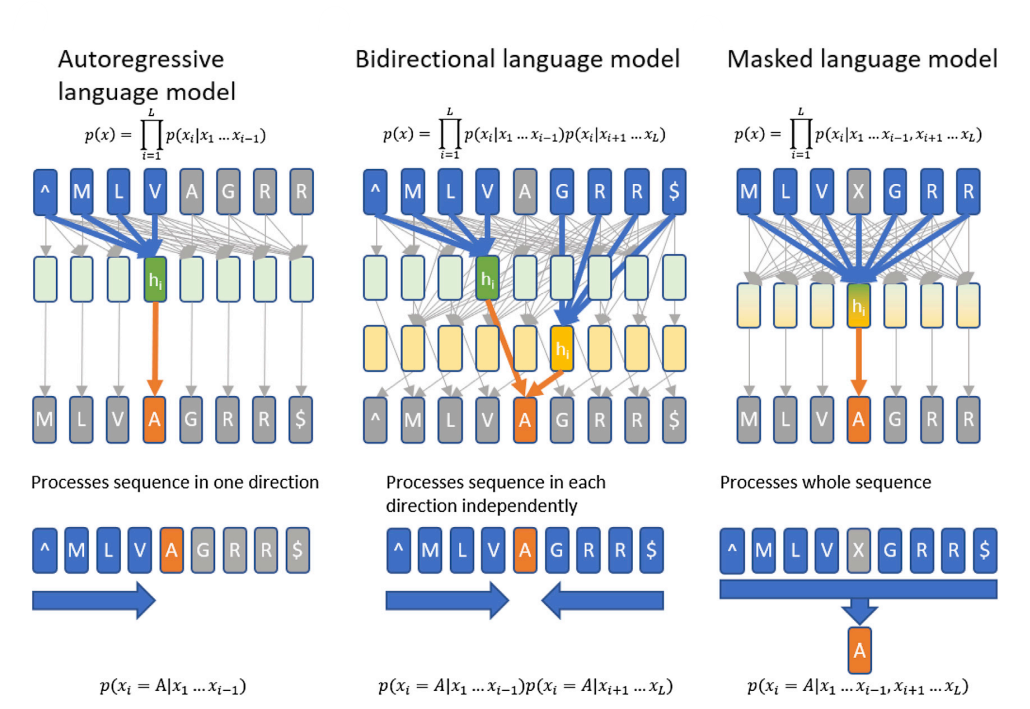
\includegraphics[scale=0.7]{rob_long_3.png}}
	\caption{A summary of the typical objective functions and neural network architectures used to solve language problems in biology. Figure taken from \cite{bepler_learning_2021}. }
	\label{figthree}
\end{figure}

While autoregressive models work well for language tasks, biological language presents a unique challenge in that context especially matters, as does the direction the sequence is analyzed. To truly 
capture the intricacies of peptide sequences, we need a different model. 

\section{ELMo and BERT: Tell Me How to Get, How to Get to a Good \\ Embedding\footnote{To learn more about ELMo, BERT, and their friends, see the following 
\href{https://www.youtube.com/watch?v=b2rBhpVDzO8&ab_channel=SesameStreet}{link}}}

Autoregressive models consider the preceding words in a sequence because the objective of the model is to predict the next word. To get a model that wants to learn context, we need a different objective 
function. The typical objective function used to improve the contextual clues a model uses for prediction tasks is called an autoencoder. It works by randomly corrupting parts of a sequence and then the 
model trains by attempting to reconstruct this sequence. 

To work with sentences, we first transform the words in the sentence into vectors in a process known as word embedding. Once a word is represented as a vector, it becomes easier to perform computations. 
A popular technique to produce these embeddings is ELMo (Embeddings from Language Models). 

\newpage
ELMo uses a bidirectional approach, meaning it considers the words to the left and right to encode semantic meaning in the vector used to represent a word. Unlike previous approaches to word embedding, 
ELMo considers the whole input sentence when deciding upon how to embed a word as a vector \cite{peters_deep_2018}. 

ELMo seems particularly well-suited for biological applications. ELMo has previously been used to detect homonyms, pairs of words that have the same spelling but different meanings depending on context 
\cite{lee_systematic_2021}. For instance, current is a homonym as it can be used in the context of current events or in the context of electrical current. Homonyms are especially important in biology. 
Because there are only 20 amino acids, amino acids tend to be reused in peptide sequences, often in different contexts \cite{bepler_learning_2021}. Furthermore, homonyms of up to 7 amino acids in length 
have been found in proteins. These homonyms exhibit different structures in different proteins, similar to how homonyms in one sentence could have a different meaning in another 
\cite{gatherer_peptide_2007}. ELMo's ability to consider contextual clues when computing word embeddings combined with its ability to distinguish between homonyms ultimately makes it well-suited for 
biological applications. 

Using ELMo, we now have vector representations of words we wish to analyze. Thus, we can finally formulate our model. Because context matters, we wish to use an autoencoder model. Formally, we let $X$ 
be a vector space of decoded messages and $Y$ be a vector space of encoded messages. By encoded messages, we mean the vector has been corrupted such that certain tokens in the original sequence were 
replaced with filler tokens. By decoding a message, our model seeks to return the original uncorrupted sequence. We represent an encoder function as $E_\phi : X \rightarrow Y$ ($E$ for encoder) and the 
decoder function as $D_\theta: Y \rightarrow X$ where $\phi$ and $\theta$ are respective parameters for our two functions. A perfect decoder, therefore, returns the original sequence after it has been 
encoded, i.e. $D_\theta(E_\phi(x)) = x$ for all $x \in X$. 


We know, however, that perfect decoders are difficult to achieve. Instead, our decoder may return another vector $x' \in X$ after encoding, i.e. there exists $x \in X$ such that $D_\theta(E_\phi(x)) = 
x'$ for some $x' \in X$. Thus, we want to train our model such that it minimizes the distance between $x'$ and $x$ in the vector space $X$. To do this, we need a function. We can therefore define our 
loss function $L$ as follows:

\begin{equation*}
    L := \frac{1}{N} \; \sum_{i = 1}^{N} \; \|x_i -D_\theta(E_\phi(x_i))\|_{2}^{2} \;,
\end{equation*}

\noindent where $N$ is the number of elements in $X$ we choose to subset, i.e. we take \\ $\{x_1, x_2, ..., x_N\} \in X$ as elements to compute our loss function \cite{noauthor_autoencoder_2023}. \\ Our 
model's task is to minimize $L$. In plain English, we wish to minimize the average distance between our original message and the reconstructed message. 

To actually train our model, we use an over complicated version of a simple principle: guess, check, and correct. We guess weights to help our encoder and decoder functions recreate the original 
sequence. Then, we check how good these weights are by computing our loss function. If our loss is high, we readjust our weights through a process known as backpropagation 
\cite{noauthor_multilayer_2023}. This process continues as we train our model.

An example of one such model is BERT, a common type of masked autoencoder model used for natural language processing (NLP) tasks \cite{he_masked_2022}. BERT utilizes a transformer architecture, a type 
of neural network, to train its model. The autoencoder objective function is \textit{what} BERT uses to train; a transformer is \textit{how} it trains \cite{devlin_bert_2018}. Transformers have two main 
features: 1) positional encoding and 2) attention. In language, order matters. Positional encoding allows a transformer to store where in a sentence each word is located to better understand its 
meaning. Attention, as the name suggests, tells the model what to pay attention to. Think about a portrait of a person. There may be trees in the background, but clearly, the focal point is the person 
in the photo. In the same way, transformers use attention as a mechanism to determine what to focus on in a sentence so as to disregard the background and less important details. 

When calculating attention, we use three inputs: queries, keys, and values, represented by the matrices $Q$, $K$, and $V$, respectively. A query is what word the model wants to focus on, similar to how 
Google search queries are used to pull up results. The query is then compared to keys, other words which may be similar to the query we wish to characterize. If the query and key are similar, their 
associated value has a higher weight. Formally, we compute attention using the following formula:

\begin{equation*}
    \textnormal{Attention}(Q, K, V) = \textnormal{softmax}\left(\frac{Q \cdot K^T}{\sqrt{d_k}}\right) V,
\end{equation*}

\noindent where $d_k$ is the dimension of the matrix $K$ \cite{vaswani_attention_2017}. 

Recall that we previously embedded words as vectors. When we take the dot product of our query and key, we're really comparing the semantic meanings of the original words. Two words with similar 
semantic meanings will embed in $Q$ and $K$ similarly, meaning the coordinates of the vectors will be similar, resulting in a larger dot product. By extension, vectors associated with two words of 
different semantic meanings are orthogonal, and thus their final weighted value is zero. A softmax function is then applied to normalize the weights. Thus, our formula for attention can be intuitively 
thought of as weighing final values based on the relative magnitude of semantic similarities between embedded words, i.e. pay attention to similar words to predict meaning. 

Once we've trained BERT, we now have a decent description of semantic similarities between sentences, or for our purposes, peptide sequences. Once a model is trained on one task, it can be used further 
on seemingly unrelated downstream tasks in a process known as transfer learning. Bepler \& Berger liken the process to how in the movie \textit{The Karate Kid}, learning how to wax on and off offers 
transferable skills in karate \cite{avildsen_karate_1984}. Biological models of BERT have a stronger ``intuition'' for how information is encoded in peptide sequences which can then be used to predict 
protein structure and function in other tasks. This ``intuition'' is encoded by the weights used to make up the functions governing the model and allows for transfer learning. Transfer learning is 
especially useful when training data is lacking, as is the case with protein function prediction. The functions of many proteins are unknown, making it difficult to accurately train a prediction model. 
However, models trained on other tasks with plentiful training data available can then be used to predict protein function successfully \cite{bepler_learning_2021}. For instance, transfer learning was 
used by Bepler \& Berger to predict which parts of a protein are inside vs. outside the cell membrane based on an initial training task of embedding peptide sequences as vectors 
\cite{bepler_learning_2019}. 

The problem with models like BERT is that this learned intuition is guarded by a black box \textemdash we don't know exactly why the model performs well at certain tasks. We only know that by learning 
the weights associated with accuracy in one task, accuracy transfers over to other tasks. To better understand the biology behind BERT's success, Vig et al. examined where BERT's transformer 
architecture places its attention \cite{vig_bertology_2020}. In one instance, they examined contact maps, a matrix $c$ where entry $c_{ij} = 1$ if amino acids $i$ and $j$ are in contact in the tertiary 
protein structure and $c_{ij} = 0$ otherwise. High attention weights above a threshold, $\theta$, were then analyzed. For an $n$-length input sequence $x$ in the model, the proportion, $p(c)$, of pairs 
of amino acids in contact with high attention can be calculated as follows:

\begin{equation*}
    p(c) = \frac{\sum\limits_{x \in X} \sum\limits_{i = 1}^{n} \sum\limits_{j = 1}^n c_{ij} \cdot \alpha_{i,j}(x)}{{\sum\limits_{x \in X} \sum\limits_{i = 1}^{n} \sum\limits_{j = 1}^n \alpha_{i,j}(x)}} 
,
\end{equation*}

where $\alpha_{i,j}(x)$ is the attention weight for the input vector $x$ between amino acids $i$ and $j$. 

The authors found that one variation of BERT for protein structure prediction, ProtBERT, contained a layer in which over 50\% of its attention was focused on contact maps. This is remarkable considering 
that ProtBERT is a language model without any spatial or topological information included in its dataset \textemdash it makes predictions purely based on peptide sequence. Furthermore, the model also 
focuses attention on amino acids which are far apart from one another in the peptide sequence but which are close together in the 3D structure (see Figure~\ref{figfour}). Thus, the model is able to 
predict the linguistic context clues we wished to encode in our model. 

\begin{figure}[h!]
	\centerline{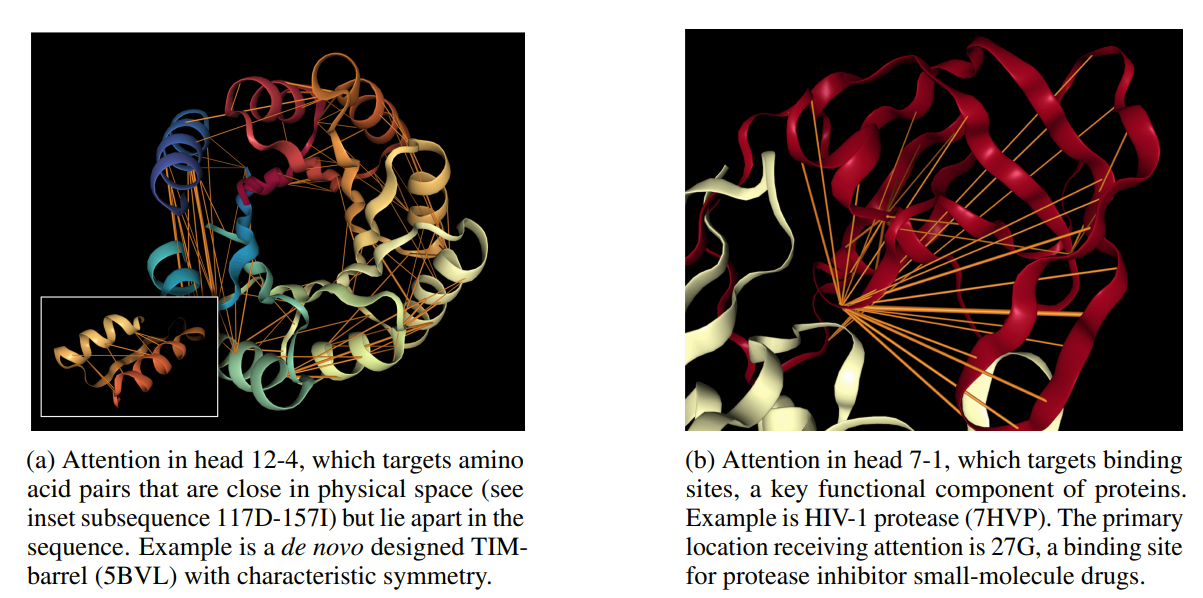
\includegraphics[scale=0.7]{rob_long_4.png}}
	\caption{Amino acids which are far apart in a peptide sequence are able to coordinate with each other in 3D. Attention in transformer models captures structural interactions between different 
amino acids. Attention also appears to highlight binding sites on proteins, which is an important feature for determining molecules that can interact with the protein. Figure taken from 
\cite{vig_bertology_2020}. }
	\label{figfour}
\end{figure}

To briefly summarize, ELMo is used to create vectors known as word embeddings which are used as inputs into autoencoder models like BERT. Because BERT is able to consider contextual information by the 
very nature of its objective function, it is able to capture valuable biological information as to how proteins fold and function. To aid in the training of this model, transformers are employed which 
use attention to disregard irrelevant information to improve accuracy. Despite these models being agnostic to topological data when training, their architecture appears to be invaluable in answering 
biological questions.  

\section{Final Thoughts}

Deciphering the code found within each of our cells is no small task. DNA becomes amino acids which become proteins \textemdash a simple and foundational idea underpinning life that only supercomputers 
seem capable of beginning to tackle. Our own communication carries with it the language found inside our cells. What is language if not the cellular language giving itself the ability to speak? Advances 
in the mathematics of language modeling have only heightened our ability to see the similarities between the protein language and our own. The protein language possesses context and meaning, where even 
one fault in the language can mean the difference between life and death. As our protein language models advance, our ability to promote human flourishing advances too. 

\newpage

\doublespacing %if needed for word count

% \section{References}
% Bibliographic references must be unambiguous and uniform.  We
% recommend giving the author names references in brackets,
% e.g. \cite{knuth1986texbook},
% \cite{boulic19913d}, \cite{dyer1995motion}, and \cite{holton1995soft}.

\bibliographystyle{plain}
\bibliography{rob_long_bib2}
  
\end{document}
